
\section{Starter File}

SS begins by reading the file starter.ss. The term COND appears in the "Typical Value" column of this documentation (it does not actually appear in the model files), it indicates that the following section is omitted except under certain conditions, or that the factors included in the following section depend upon certain conditions. In most cases, the description in the definition column is the same as the label output to the ss\_new files.

{
\setlength\extrarowheight{4pt}
\begin{landscape}
\subsection{Starter File Options (starter.ss)}	
%\centerline{\large{STARTER.SS}} 
%\vspace{0.1in}
%{\renewcommand{\arraystretch}{1.1}

\begin{longtable}{p{1.5cm} p{7.2cm} p{12.3cm}} 

 \hline
 \textbf{Value} & \textbf{Options} & \textbf{Description} \TBstrut \\ 
 \hline
 \endfirsthead
 
 \hline
 \textbf{Value} & \textbf{Options} & \textbf{Description} \TBstrut \\ 
 \hline
 \endhead
 
 \hline
 \endfoot
 
 \hline
 \multicolumn{3}{ c }{ \textbf{End of Starter File}}\Tstrut\Bstrut\\
 \hline
 \endlastfoot

 \#C this is a starter comment & Must begin with \#C then rest of the line is free form & All lines in this file beginning with \#C will be retained and written to the top of several output files \Tstrut\\
		
 \hline
 data\textunderscore file.dat &  & File name of the data file \Tstrut\\
		
 \hline
 control\textunderscore file.ctl &  & File name of the control file \Tstrut\\
   
 \hline		
 0 & Initial Parameter Values: & \multirow{1}{1cm}[-0.25cm]{\parbox{12.5cm}{Do not set equal to 1 if there have been any changes to the control file that would alter the number or order of parameters stored in the ss.par file.  Values in ss.par can be edited, carefully. Do not run ss\_trans.exe from a ss.par from SS v.3.24.}}\Tstrut\\
 & 0 = use values in control file; and&  \\
 & 1 = use ss.par after reading setup in the control file. & \\
		
 \hline
 1 & Run display detail: &  \multirow{1}{1cm}[-0.25cm]{\parbox{12.5cm}{With option 2, the display shows value of each -logL component for each iteration and it displays where crash penalties are created}} \Tstrut\\
   & 0 = none other than ADMB outputs; & \\
   & 1 = one brief line of display for each iteration; and & \\
   & 2 = fuller display per iteration. & \\
		  
 \hline
 1 & Detailed age-structure report: & \multirow{1}{1cm}[-0.15cm]{\parbox{12.5cm}{Option 0 will forgo the writing of the Report file, but the ss\_summary file will be written that has minimal derived and estimated quantities. This is a useful option for some data-limited assessment approaches (e.g., XSSS or SSS). Option 1 will write out the full Report file. Option 2 will write out select items in the Report file and will omit some more detailed sections (e.g., numbers-at-age).}} \Tstrut\\
   & 0 = minimal (no Report file); & \\
   & 1 = include all output; and &  \\
   & 2 = brief output. &  \\	
   & & \\	 
		 
 \pagebreak%\hline
 0 & Write 1st iteration details: & \multirow{1}{1cm}[-0.25cm]{\parbox{12.5cm}{This output is largely unformatted and undocumented and is mostly used by the developer. }} \Tstrut\\
   & 0 = omit; and & \\
   & 1 = write detailed intermediate calculations to echoinput.sso during first call. & \\

 \hline
 0 & Parameter Trace: & \multirow{1}{1cm}[-0.25cm]{\parbox{12.5cm}{This controls the output to parmtrace.sso. The contents of this output can be used to determine which values are changing when a model approaches a crash condition.  It also can be used to investigate patterns of parameter changes as model convergence slowly moves along a ridge.}} \Tstrut\\
   & 0 = omit; & \\
   & 1 = write good iteration and active parameters; & \\
   & 2 = write good iterations and all parameters; & \\
   & 3 = write every iteration and all parameters; and & \\
   & 4 = write every iteration and active parameters. &  \\
   
 \hline
 1 & Cumulative Report: & \multirow{1}{1cm}[-0.25cm]{\parbox{12.5cm}{Controls reporting to the file Cumreport.sso.
 		This cumulative report is most useful when accumulating summary information from likelihood profiles or when simply accumulating a record of all model runs within the current subdirectory}}\Tstrut\\
   & 0 = omit;  & \\
   & 1 = brief; and & \\
   & 2 = full.  &  \\
	 
 \hline
 1 & Full Priors: & \multirow{1}{1cm}[-0.25cm]{\parbox{12.5cm}{Turning this option on (1) adds the log likelihood contribution from all prior values for fixed and estimated parameters to the total negative log likelihood.  With this option off (0), the total negative log likelihood will include the log likelihood for priors for only estimated parameters.}} \Tstrut\\
   & 0 = only calculate priors for active parameters; and &	\\
   & 1 = calculate priors for all parameters that have a defined prior. & \\
	     
 %\hline
 \pagebreak
 1 & Soft Bounds: & \multirow{1}{1cm}[-0.25cm]{\parbox{12.5cm}{This option creates a weak symmetric beta penalty for the selectivity parameters.  This becomes important when estimating selectivity functions in which the values of some parameters cause other parameters to have negligible gradients, or when bounds have been set too widely such that a parameter drifts into a region in which it has negligible gradient.  The soft bound creates a weak penalty to move parameters away from the bounds.}} \Tstrut\\
   & 0 = omit; and & \\
   & 1 = use. & \\
   & & \\
   & & \\
   & & \\

 
 \hline
 1 & Data File Output: & \multirow{1}{1cm}[-0.25cm]{\parbox{12.5cm}{All output files are sequentially output to data.ss\_new and will need to be parsed by the user into separate data files. The output of the input data file makes no changes, so retains the order of the original file. Output files 2-N contain only observations that have not been excluded through use of the negative year denotation, and the order of these output observations is as processed by the model. The N obs values are adjusted accordingly.  At this time, the tag recapture data is not output to data.ss\_new.}}\Tstrut\\
   & 0 = none; & \\
   & 1 = output an annotated replicate of the input data file; & \\
   & 2 = add a second data file containing the model's expected values with no added error; and & \\
   & 3+ = add N-2 parametric bootstrap data files. & \\

 \hline
 8 & Turn off estimation: &  \multirow{1}{1cm}[-0.25cm]{\parbox{12.5cm}{The 0 option is useful for (1) quickly reading in a messy set of input files and producing the annotated control.ss\_new and data.ss\_new files, or (2) examining model output based solely on input parameter values.  Similarly, the value option allows examination of model output after completing a specified phase.  Also see usage note for restarting from a specified phase.}}\Tstrut\\
   & -1 = exit after reading input files; & \\
   & 0 = exit after one call to the calculation routines and production of sso and ss\_new files; and & \\
   & <positive value> = exit after completing this phase. & \\	  
	     
 \hline
 1000 & MCMC burn interval & Number of iterations to discard at the start of an MCMC run. \Tstrut\\
	   
 \hline
 200 & MCMC thin interval & Number of iterations to remove between the main period of the MCMC run. \Tstrut\\
	   
 %\hline 
 0.0 & \hyperlink{Jitter}{Jitter:} & \multirow{1}{1cm}[-0.25cm]{\parbox{12.5cm}{The jitter function has been revised with SS v.3.30.  Starting values are now jittered based on a normal distribution with the pr(P\textsubscript{MIN}) = 0.1\% and the pr(P\textsubscript{MAX}) = 99.9\%. A positive value here will add a small random jitter to the initial parameter values.  When using the jitter option, care should be given when defining the low and high bounds for parameter values and particularly -999 or 999 should not be used to define bounds for estimated parameters.}}\Tstrut\\ 
	 & 0 = no jitter done to starting values; and & \\
	 & >0 starting values will vary with larger jitter values resulting in larger changes from the parameter values in the control or par file. & \\
	 & & \\
	
 \hline
 -1 & SD Report Start: & \Tstrut\\
    & -1 = begin annual SD report in start year; and & \\
    & <year> = begin SD report this year. & \\
	      
 \hline
 %\pagebreak
 -1 & SD Report End: & \Tstrut\\
    & -1 = end annual SD report in end year; & \\
    & -2 = end annual SD report in last forecast year; and & \\
    & <value> = end SD report in this year. & \\
	   
 \hline
 2 & Extra SD Report Years: & \multirow{1}{1cm}[-0.25cm]{\parbox{12.5cm}{In a long time series application, the model variance calculations will be smaller and faster if not all years are included in the SD reporting.  For example, the annual SD reporting could start in 1960 and the extra option could select reporting in each decade before then.}}\Tstrut\\
   & 0 = none; and & \\
   & <value> = number of years to read. &  \\
   & & \\

 %\pagebreak 
 \hline  
 \multicolumn{3}{l}{COND: If Extra SD report years > 0} \Tstrut\\

 %\pagebreak
 \hline
 \multicolumn{1}{r}{1940 1950} & \multirow{1}{1cm}[-0.25cm]{\parbox{19.5cm}{Vector of years for additional SD reporting. The number of years need to equal the value specified in the above line (Extra SD Reporting). }} \Tstrut\\
 & & \\

 \pagebreak 
 %\hline
 0.0001 & Final convergence & \multirow{1}{1cm}[-0.25cm]{\parbox{12.5cm}{This is a reasonable default value for the change in log likelihood denoting convergence.  For applications with much data and thus a large total log likelihood value, a larger convergence criterion may still provide acceptable convergence}}\Tstrut\\
        & & \\
        & & \\
		& & \\ 
 
 \hline
 0 & Retrospective year: & \multirow{1}{1cm}[-0.25cm]{\parbox{12.5cm}{Adjusts the model end year and disregards data after this year.  May not handle time varying parameters completely.}} \Tstrut\\
   & 0 = none; and & \\
   & -x = retrospective year relative to end year. & \\
  
 \hline
 0 & Summary biomass min age & \multirow{1}{1cm}[-0.25cm]{\parbox{12.5cm}{Minimum integer age for inclusion in the summary biomass used for reporting and for calculation of total exploitation rate.}}\Tstrut\\
   & & \\ 

 \hline
 %\pagebreak
 1 & Depletion basis: & \multirow{1}{1cm}[-0.25cm]{\parbox{12.5cm}{Selects the basis for the denominator when calculating degree of depletion in SB.  The calculated values are reported to the SD report.}}\Tstrut\\
   & 0 = skip; & \\
   & 1 = X*SB0; & Relative to virgin spawning biomass.\\
   & 2 = X*SB\textsubscript{MSY}; & Relative to spawning biomass that achieves MSY.\\
   & 3 = X*SB\textsubscript{styr}; and & Relative to model start year spawning biomass.\\
   & 4 = X*SB\textsubscript{endyr}. & Relative to spawning biomass in the model end year.\\
  
 \hline
 1 & Fraction (X) for depletion denominator & Value for use in the calculation of the ratio for SSB\textsubscript{y}/(X*SSB0).\Tstrut\\

 \hline
 %\pagebreak
 1 & SPR report basis: & \multirow{1}{1cm}[-0.25cm]{\parbox{12.5cm}{SPR is the equilibrium SSB per recruit that would result from the current year’s pattern and intensity of F’s.  The quantities identified by 1, 2, and 3 here are all calculated in the benchmarks section.  Then the one specified here is used as the selected }}\Tstrut\\
   & 0 = skip; & \\
   & 1 = use 1-SPR\textsubscript{target}; & \\
   & 2 = use 1-SPR at MSY; & \Tstrut\\
 
 \pagebreak
   & 3 = use 1-SPR at B\textsubscript{target}; and & \multirow{1}{1cm}[-0.25cm]{\parbox{12.5cm}{Denominator in a ratio with the annual value of (1 – SPR). This ratio (and its variance) is reported to the SD report output for the years selected above in the SD report year selection.}}\Tstrut\\
   & 4 = no denominator, so report actual 1-SPR values. & \\
  
 %\pagebreak
 \hline 
 4 & F std report value: &  \multirow{1}{1cm}[-0.25cm]{\parbox{12.5cm}{In addition to SPR, an additional proxy for annual F can be specified here.  As with SPR, the selected quantity will be calculated annually and in the benchmarks section.  The ratio of the annual value to the selected (see F report basis below) benchmark value is reported to the SD report vector.  Options 1 and 2 use total catch for the year and summary abundance at the beginning of the year, so combines seasons and areas.  But if most catch occurs in one area and there is little movement between areas, this ratio is not informative about the F in the area where the catch is occurring.  Option 3 is a simple sum of the full F’s by fleet, so may provide non-intuitive results when there are multi areas or seasons or when the selectivities by fleet do not have good overlap in age.  Option 4 is a real annual F calculated as a numbers weighted F for a specified range of ages (read below).  The F is calculated as Z-M where Z and M are each calculated an ln(N\textsubscript{t+1}/N\textsubscript{t}) with and without F active, respectively. The numbers are summed over all biology morphs and all areas for the beginning of the year, so subsumes any seasonal pattern.}}\Tstrut\\
   & 0 = skip; & \\
   & 1 = exploitation rate in biomass; & \\
   & 2 = exploitation rate in numbers; & \\

   & 3 = sum(full F's by fleet); & \\
   & 4 = population F for range of ages; and & \\
   & 5 = unweighted average F for range of ages. & \\
   & & \\
   & & \\
   & & \\
   & & \\
   & & \\ 
  
 \hline
 %\pagebreak
 \multicolumn{2}{l}{COND: If F std reporting $\geq$ 4 } & \multirow{1}{1cm}[-0.25cm]{\parbox{12.5cm}{Specify range of ages. Upper age must be less than max age because of incomplete handling of the accumulator age for this calculation.}} \Tstrut\\

 \multicolumn{1}{r}{13 17}  & Age range if F std reporting = 4. & \Tstrut\\

 \hline
 %\pagebreak
 1 & F report basis: &  \multirow{1}{1cm}[-0.25cm]{\parbox{12.5cm}{Selects the denominator to use when reporting the F std report values.  Note that order of these options differs from the biomass report basis options.}}\Tstrut\\
   & 0 = not relative, report raw values; & \\
   & 1 = use F std value corresponding to SPR\textsubscript{target}; & \\
   & 2 = use F std value corresponding to F\textsubscript{MSY}; and & \\
 
  \pagebreak
   & 3 = use F std value corresponding to F\textsubscript{Btarget}. & \Tstrut\\

  \hline
  %\pagebreak
  0.01 & MCMC output detail: & \multirow{1}{1cm}[-0.25cm]{\parbox{12.5cm}{Specify format of MCMC output. This input requires the specification of two items; the output detail and a bump value to be added to the ln(R0) in the first call to MCMC. A bias adjustment of 1.0 is applied to recruitment deviations in the MCMC phase, which could result in reduced recruitment estimates relative to the MLE when a lower bias adjustment value is applied.  A small value, called the "bump", is added to the ln(R0) for the first call to MCMC in order to prevent the stock from hitting the lower bounds when switching from MLE to MCMC. If you wanted to select the default output option and apply a bump value of 0.01 this is specified by 0.01 where the integer value represents the output detail and the decimal is the bump value.}} \Tstrut\\
  & 0 = default; & \\
  & 1 = output likelihood components and associated lambda values; &  \\
  & 2 = expanded output; and &  \\		 
  & 3 = make output subdirectory for each MCMC vector. &  \\
  & & \\
  & & \\  		 
  
  \hline
  \hypertarget{ALK}{0} & Age-length-key (ALK) tolerance level, 0 >= values required & \multirow{1}{1cm}[-0.25cm]{\parbox{12.5cm}{Value of 0 will not apply any compression.  Values > 0 (e.g. 0.0001) will apply compression to the ALK which will increase the speed of calculations.  The size of this value will impact the run time of your model, but one should be careful to ensure that the value used does not appreciably impact the estimated quantities relative to no compression of the ALK.  The suggested value if applied is 0.0001.}} \Tstrut\\ 
  & & \\
  & & \\
  & & \Bstrut\\
  
  \hline  
  \multicolumn{2}{l}{COND: Seed Value}& \multirow{1}{1cm}[-0.25cm]{\parbox{12.5cm}{This is an optional input value which allows for the specification of a random number seed value.  If you do not with to specify a seed, skip this input line and end the reading of the starter file with the check value (3.30). }} \Tstrut\\
  & & \\ 
  & & \\
  \multicolumn{1}{r}{123} & Set seed value: & \multirow{1}{1cm}[-0.25cm]{\parbox{12.5cm}{Specify a seed for data generation. This feature is not available in versions prior to 3.30.15.}}\\ 
  & & \Tstrut\\
  
  \pagebreak
 %\hline
 \hypertarget{Convert}{3.30} & Model version check value. & \multirow{1}{1cm}[-0.25cm]{\parbox{12.5cm}{ A value of 3.30 indicates that the control and data files are currently in SS v3.30 format and a value of 999 indicates that the control and data file are in a previous SS v.3.24 version. The ss\_trans.exe executable should be used and will convert the 3.24 version files to the new format in the control.ss\_new and data.ss\_new files.  All ss\_new files are in the SS v.3.30 format, so starter.ss\_new has SS v.3.30 on the last line.  The mortality-growth parameter section has a new sequence, so SS v.3.30 cannot read a ss.par file produced by SS v.3.24 and earlier, so please ensure that read par file option at the top of the starter file is set to 0. The \hypertarget{ConvIssues}  {Converting Files from SS v.3.24} section has additional information on model features that may impede file conversion.}}\Tstrut\\
     & & \\  
     & & \\  
	 & & \\
     & & \\
   	 & & \\
     & & \\  
     & & \\  
     & & \\       
\end{longtable}
\end{landscape}
}
\restoregeometry

\subsection{Jitter}
\hypertarget{Jitter}{}
The jitter function has been updated with SS v.3.30.  The following steps are now performed to determine the jittered starting parameter values (illustrated in the figure below):
\begin{enumerate}
	\item A normal distribution is calculated such that the pr(P\textsubscript{MIN}) = 0.1\% and the pr(P\textsubscript{MAX}) = 99.9\%.
	\item A jitter shift value, termed "\textit{K}", is calculated from the distribution equal to pr(P\textsubscript{CURRENT}).
	\item A random value is drawn, "\textit{J}", from the range of \textit{K}-jitter to \textit{K}+jitter.
        \item Any value which falls outside the 0-1 range (in the cumulative normal space) is mapped back from the bound to a point one-tenth of the way from the bound to the initial value.
	\item \textit{J} is a new cumulative normal probability value.
	\item Calculate a new parameter value, P\textsubscript{JITTERED}, such that pr(P\textsubscript{JITTERED}) = \textit{J}.
\end{enumerate}


\begin{center}
	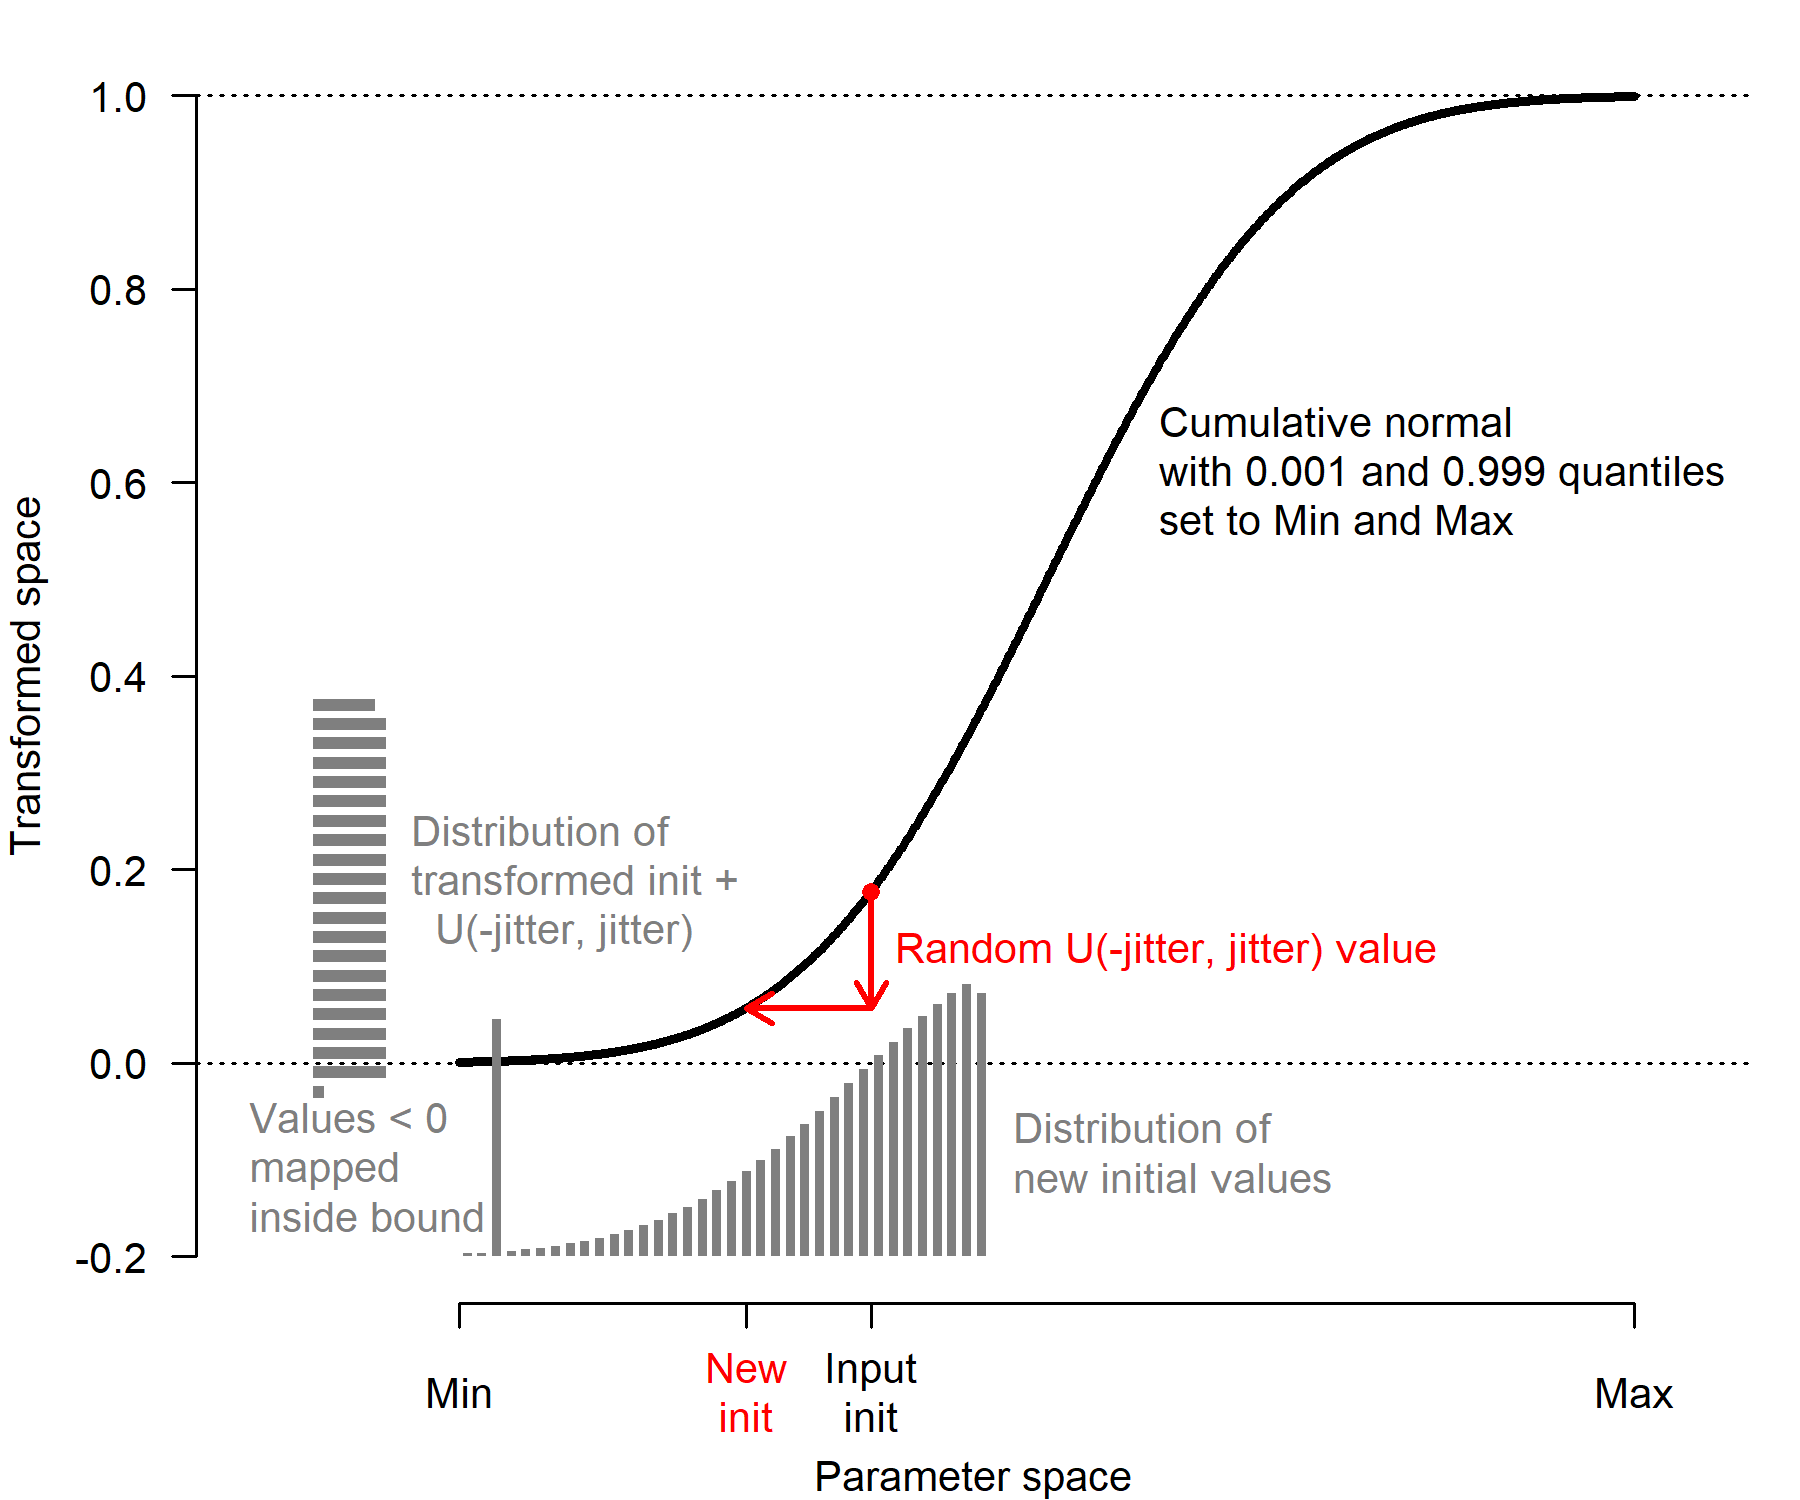
\includegraphics[scale = 0.75]{jitter_illustration}\\
	Illustration of the jitter algorithm
\end{center}


In SS, the jitter fraction defines a uniform distribution in cumulative normal space +/- the jitter fraction from the initial value (in cumulative normal space). The normal distribution for each parameter, for this purpose, is defined such that the minimum bound is at 0.001, and the maximum at 0.999 of the cumulative distribution. If the jitter faction and original initial value are such that a portion of the uniform distribution goes beyond 0.001 or 0.999 of the cumulative normal, the new value is set to one-tenth of the way from the bound to the original initial value. 

Therefore sigma = (max-min) / 6.18. For parameters that are on the log-scale, sigma may be the correct measure of variation for jitters, for real-space parameters, CV (= sigma/original initial value) may be a better measure. 

If the original initial value is at or near the middle of the min-max range, then for each 0.1 of jitter, the range of jitters extends about 0.25 sigmas to either side of the original value (though as the total jitter increases the relationship varies more than this), and the average absolute jitter is about half of that.  For values far from the middle of the min-max range, the resulting jitter is skewed in parameter space, and may hit the bound, invoking the resetting mentioned above. 

To evaluate the jittering, the bounds, and the original initial values, a jitter\_info table is available from r4ss, including sigma, CV and InitLocation columns (the latter referring to location within the cumulative normal – too close to 0 or 1 indicates a potential issue).

Note: parameters with min $\leq$ -99 or max $\geq$ 999 are not jittered to avoid unreasonable values (a warning is produced to indicate this).

\pagebreak
